%
% dgl.tex -- Einige Informationen über Differentialgleichungen
%
% (c) 2018 Prof Dr Andreas Müller, Hochschule Rapperswil
%
\chapter{Differentiagleichungen\label{chapter:dgl}}
\lhead{Kapitel 3: Differentialgleichungen}
Modelle für das Klima oder für einzelne Teilaspekte des Klimas 
werden häufig in der Form einer Differentialgleichung formuliert.
Die kurzfristigen Schwankungen einer Lösung entsprechen 
eher den Wettererscheinungen, die für unsere Betrachtungen nicht
interessant sind.
Für Klima-Betrachtungen suchen wir Lösungen der Differentialgleichungen,
die über lange Zeit konstant sind, sogenannte Gleichgewichtslösungen.
Diese werden natürlich von Parametern wie der $\text{CO}_2$-Konzentration
oder dem Salzgehalt der Meere abhängig sein.
Die interessante Frage wird daher sein, wie sich die Gleichgewichtslösungen
verändern, wenn die Parameter sich ändern.

In diesem Kapitel sollen die wichtigsten Eigenschaften von
Vektor-Differentialgleichungen und der einfachsten Bifurkationen
zusammengestellt werden.
Das Thema Differentialgleichungen wurde 2016 im Mathematischen Seminar
behandelt.
Das Seminar-Buch \cite{skript:mathsem-dgl} enthält eine vertiefte Diskussion
der Theorie.

%
% dgl.tex
%
% (c) 2018 Prof Dr Andreas Müller, Hochschule Rapperswil
%
\section{Grundlagen}
\rhead{Grundlagen}
Eine Differentialgleichung ist eine Beziehung zwischen einer Funktion und
ihren Ableitungen.
Wir betrachten Funktionen der Zeit $t$ mit Werten in $\mathbb R^n$
und schreiben sie $x(t)$.
Sei $f$ eine Funktion
\[
f\colon \mathbb R^n\times \mathbb R \to \mathbb R^n: (x,t) \mapsto f(x,t).
\]

\begin{definition}
Eine Funktion $x(t)$ heisst Lösung der Differentialgleichung
\begin{equation}
\frac{dx}{dt} = f(x,t)
\label{skript:dgl:dgldef}
\end{equation}
zur Anfangsbedingung $x_0$, wenn gilt $x(0)=x_0$ und
\[
\frac{dx(t)}{dt} = f(x(t),t)
\]
für alle $t>0$.
\end{definition}

Unter einigermassen milden Bedingungen an die Funktion $f(x,t)$ ist
sichergestellt, dass eine Differentialgleichung immer eine Lösung hat.

\subsection{Autonome Differentialgleichungen}
Wenn die Funktion $f$ von der Zeit abhängt, wird es im allgemeinen
keine konstanten Lösungen geben.
Für die Klimadiskussion sind wir allerdings daran interessiert, ob
ein Modell Lösungen hat, die sich mit der Zeit nicht ändern.
Solche Lösungen zeigen uns, dass wir alle kurzfristigen
Schwankungen, die wir dem Wetter zuordnen würden, ausgemittelt haben.

\begin{definition}
Eine Differentialgleichung der Form~\eqref{skript:dgl:dgldef}
heisst {\em autonom},
\index{autonom}%
wenn die Funktion $f$ nicht von der Zeit abhängt.
Eine autonome Differentialgleichung kann als
\[
\frac{dx}{dt} = f(x)
\]
geschrieben werden.
\end{definition}

\subsection{Umwandlung in eine autonome Differentialgleichung}
Die Forderung, dass die Differentialgleichung autonom sein soll, ist
auf triviale Art erfüllbar, indem man zu einer neuen
unabhängigen Variablen $s$ übergeht und die bisherige Zeitvariable 
als letzte Komponente der Vektorfunktion $x(t)$ hinzufügt.

Wir schreiben die Lösungsfunktionen als
\begin{align*}
x(t)
&=
\begin{pmatrix}
x_1(t) \\ \vdots \\x_n(t)
\end{pmatrix}
&&\text{und erweitern dies zu}&
\bar x(s)
=
\begin{pmatrix}
x_1(s) \\ \vdots \\ x_n(s) \\ s
\end{pmatrix}
\in\mathbb R^{n+1}.
\end{align*}
Die rechte Seite der Differentialgleichung, also die Funktion $f(x,t)$
schreiben wir
\begin{align*}
f(x,t)
&=
f(x_1,\dots,x_n,t)
&&\text{mit Anfangsbedingung}&
x_0
&=
\begin{pmatrix} x_{01} \\ \vdots \\ x_{0n} \end{pmatrix}
\\
\intertext{und erweitern dies nun zu einer Funktion $\bar f$ für eine
autonome Differentialgleichung für $\bar x$}
\bar f(\bar x)
&=
\begin{pmatrix}
f_1(\bar x_1,\dots,\bar x_n,\bar x_{n+1})\\
\vdots\\
f_n(\bar x_1,\dots,\bar x_n,\bar x_{n+1})\\
1
\end{pmatrix}
&&\text{mit Anfangsbedingung}&
\bar x_0
&=
\begin{pmatrix} x_{01} \\ \vdots \\ x_{0n} \\ 0\end{pmatrix}.
\end{align*}
Die Differentialgleichung für $\bar x$ ist
\begin{equation}
\frac{d\bar x}{ds}
=
\bar f(\bar x),
\label{skript:dgl:autodgl}
\end{equation}
dies ist offensichtlich eine autonome Differentialgleichung.
Die letzte Komponenten von \eqref{skript:dgl:autodgl} ist die
Differentialgleichung für $\bar x_{n+1}$
\[
\frac{d\bar x_{n+1}}{ds} = 1
\]
mit der Anfangsbedingung $x_{n+1}(0)=0$, sie hat die Lösung
$\bar x_{n+1}(s)=s$.
Die Koordinate $\bar x_{n+1}$ ist also nichts anderes als die
ursprüngliche Zeitkoordinate.
Aus der Lösung $\bar x(s)$ der autonomen Differentialgleichung
kann die Lösung der ursprünglichen Differentialgleichung gewonnen
werden, indem man einfach die letzte Koordinate weg lässt:
\[
x(t)
=
\begin{pmatrix}
\bar x_1(t) \\ \vdots \\ \bar x_n(t)
\end{pmatrix}.
\]
Der Übergang zur autonomen Differentialgleichung erhöht die Dimension
des Vektors.
Dadurch wird die Diskussion kritischer Punkte und Gleichgewichtslösungen
leider nicht vereinfacht.
Statt eine Differentialgleichung nachträglich autonom zu machen
ist daher im allgemeinen anzustreben, dass sie von vornherein
autonom ist.
In den nachfolgenden Beispielen gehen wir daher immer von autonomen
Differentialgleichungssystemen aus.




%
% crit.tex
%
% (c) 2018 Prof Dr Andreas Müller, Hochschule Rapperswil
%
\section{Gleichgewichtslösungen und kritische Punkte}
\rhead{Gleichgewichtslösungen}
Wir gehen in diesem Abschnitt von einer autonomen Differentialgleichung
der Form
\begin{equation}
\frac{dx}{dt} = f(x)
\label{skript:dgl:gleichung}
\end{equation}
aus
mit einer Funktion $f\colon \mathbb R^n \to \mathbb R^n$.
Die Funktion $f$ wird im Allgemeinen von weiteren Parametern abhängen
wie zum Beispiel dem $\text{CO}_2$-Gehalt der Atmosphäre oder der Salinität
der Meere.
Sofern nötig machen wir diese mit der Schreibweise $f(x,p)$ mit
$p\in\mathbb R^m$ explizit sichtbar.

\begin{definition}
Ein Punkt $x_0\in\mathbb R^n$ heisst {\em Gleichgewichtslösung}
wenn die konstante Funktion $x(t)=x_0$ eine Lösung der
Differentialgleichung~\ref{skript:dgl:gleichung} ist.
\index{Gleichgewichtslösung}
\end{definition}

Eine Gleichgewichtslösung hat $\dot{x}(t)=0$ und ist daher eine
Nullstelle der Funktion $f$,
$f(x_0)=0$.
\begin{definition}
Eine Nullstelle von $f$ heisst {\em kritischer Punkt} der
Differentialgleichung~\ref{skript:dgl:gleichung}.
\end{definition}
\index{kritischer Punkt}%

Wenn $f$ ausserdem von den Parametern $p\in\mathbb R^m$ abhängt,
wird auch die Menge der Nullstellen von $f$ von $p$ abhängen.
Wir schreiben
\[
N(p) = \{x\in\mathbb R^n\;|\; f(x,p)\}
\]
für die Menge der Nullstellen. 
Im Allgemeinen werden sich die Mengen $N(p)$ für verschiedene $p$ 
unterscheiden.

Sei also $p_0\in\mathbb R^m$ ein Parametervektor und $x_0$ eine
Gleichgewichtslösung von $f$, also $f(x_0,p_0)=0$.
Unter zusätzlichen Annahmen über die Funktion $f$ kann man zeigen,
dass $x_0$ in einer Umgebung von $p_0$ zu einer Funktion
$x_0(p)$ erweitert werden kann, derart dass $x_0(p)$ jeweils ein
kritischer Punkt von $f$ ist für die Parameterwerte $p$, also
$f(x_0(p),p)=0$.
Diese Theorie ist für allerdings nicht besonders nützlich, denn
sie sagt uns nur, dass sich kritische Punkte stetig in Abhängigkeit vom
Parametervektor bewegen.
Besonders interessant für die Diskussion des Klimawandels sind
Fälle, wo Gleichgewichtslösungen sich sprunghaft ändern, wie wir in
Abschnitt~\ref{subsection:budyko} diskutieren werden.

\subsection{Stabilität}
Wir betrachten eine Gleichgewichtslösung $x(t)=x_0$ der Differentialgleichung
\eqref{skript:dgl:gleichung}.
\begin{definition}
Die Gleichgewichtslösung $x(t)=x_0$ heisst stabil, wenn eine Lösung zu
einer Anfangsbedingung $\bar x_0$, die $|x_0-\bar x_0|<\varepsilon$
erfüllt, für alle Zeiten nahe bei $x_0$ bleibt, also
$|\bar x(t)- x_0|<\varepsilon$.
\end{definition}
\index{Stabilität}%

\begin{beispiel}
Wir betrachten die Differentialgleichung
\[
\frac{dx}{dt} = ax.
\]
Sie hat die Gleichgewichtslösung $x(t)=0$.
Eine Lösung, die die Anfangsbedingung $x(0)=\varepsilon$ erfüllt, 
ist $x(t)=\varepsilon e^{at}$, denn
\[
\frac{d}{dt}
\varepsilon e^{at}
=
a\varepsilon e^{at}.
\]
Wenn $a>0$, dann wächst die Lösung exponentiell an, die Gleichgewichtslösung 
ist als nicht stabil.
Für $a<0$ dagegen nimmt $x(t)=\varepsilon e^{at}$ exponentiell schnell ab,
die Gleichgewichtslösung ist stabil.
\end{beispiel}

Für eindimensionale Systeme ist Stabilität besonders einfach zu
diskutieren, wir tun dies im Rahmen der Diskussion der wichtigsten
Bifurkationstypen in Abschnitt~\ref{section:bifurkation-eindim}.

\subsection{Zeitumkehr}
\index{Zeitumkehr}%
Wir gehen wieder von der autonomen
Differentialgleichung~\eqref{skript:dgl:gleichung}
mit der Lösung $x(t)$ mit Anfangsbedingung $x_0$ aus.
Ersetzen wir $t$ durch $-s$, erhalten wir die autonome Differentialgleichung
\begin{equation}
-\frac{dx}{ds}
=
f(x),
\end{equation}
mit der gleichen Anfangsbedingung.
Die Funktion $s\mapsto x(-s)$ ist eine Lösung.

Die Zeitumkehr verändert den Stabilitätscharakter einer Gleichgewichtslösung.
Ist $x_0$ eine stabile Gleichgewichtslösung, dann nehmen Lösungen mit
Anfangsbedingungen in der Nähe von $x_0$ nicht weiter zu, sondern
höchstens ab.
Es ist also möglich, dass die Lösung nach Zeitumkehr instabil wird.

Bei zweidimensionalen Systemen ist es aber durchaus möglich, eine
Gleichgewichtslösung in beiden Zeitrichtungen instabil sind.
Als Beispiel betrachten wir das zweidimensionale Differentialgleichungssystem
\begin{equation}
\frac{d}{dt}
\begin{pmatrix}x\\y\end{pmatrix}
=
\begin{pmatrix}1&0\\0&-1\end{pmatrix}
\begin{pmatrix}x\\y\end{pmatrix}.
\end{equation}
Sie hat die beiden Lösungen
\begin{align*}
x_1(t)&=
\varepsilon \begin{pmatrix}e^t\\0\end{pmatrix}
&&\text{und}&
x_2(t)
&=
\varepsilon \begin{pmatrix}0\\e^{-t}\end{pmatrix}
\end{align*}
zu den Anfangsbedingungen
\begin{align*}
x_1(0)&=\begin{pmatrix}\varepsilon\\0\end{pmatrix}
&&\text{und}&
x_2(0)&=\begin{pmatrix}0\\\varepsilon\end{pmatrix}.
\end{align*}
Die Lösung $x_1(t)$ wächst für $t>0$ exponentiell an, die Gleichgewichtslösung
$x(t)=0$ kann also für $t>0$ nicht stabil sein.
Für $t\to-\infty$ nimmt $x_1(t)$ exponentiell ab, aber trotzdem ist
die Nulllösung nicht stabil, dann die Lösung $x_2(t)$ nimmt für 
$t\to-\infty$ exponentiell zu.

\section{Bifurkationen eindimensionaler Systeme
\label{section:bifurkation-eindim}}
In diesem Abschnitt betrachten wir eindimensionale Differentialgleichung
\begin{equation}
\frac{dx}{dt} = f(x,\lambda),
\end{equation}
die ausserdem von einem Parameter $\lambda$ abhängt.
Wir fragen nach den Gleichgewichtslösungen in Abhängigkeit vom
Parameter $\lambda$.

\rhead{Bifurkationen}
Die nachfolgenden prototypischen Bifurkationen können in vielen
\index{Bifurkation}%
weiteren Differentialgleichungen beobachtet werden. 
Für alle Werte des Parameters ist $0$ ein kritischer Wert,
es gilt also $f(0,\lambda)=0$.
Wir können die $f$ in eine Taylor-Reihe 
\begin{equation}
f(x,\lambda)
=
\sum_{k,l} \frac{1}{(k+l)!}\frac{\partial^{k+l} f(0,0)}{\partial t^k\partial\lambda^l} x^k\lambda^l
=
a_{10}x + a_{01}\lambda
+
a_{20}x^2 + a_{11}x\lambda + a_{02}\lambda^2 + \dots
\end{equation}
entwickeln.
Die verschiedenen Bifurkationen lassen sich charakterisieren durch
die führenden Terme in dieser Entwicklung.
Insbesondere können wir verlangen, dass der führende Term für $\lambda$
immer linear in $\lambda$ sein soll.
Ist dies nämlich nicht der Fall, ist also der führende Term in 
$\lambda$ von der Form $\lambda^\alpha$, ersetzen wir den
Parameter einfach durch $\tau=\lambda^\alpha$.

In den folgenden Beispielen und Abschnitten wird der Parameter $\lambda$
entlang der horizontalen Achse aufgezeichnet, die Position $x$
entlang der vertikalen Achse.
Positive Werte von $f(x,\lambda)$ führen dazu, dass sich mit zunehmender
Zeit die Lösung $x(t)$ nach oben bewegt, solche Punkte werden in den
Diagrammen rot eingefärbt, ausserdem wird mit Pfeilen die Bewegungsrichtung
der Punkte angedeutet.

\begin{beispiel}
\begin{figure}
\centering
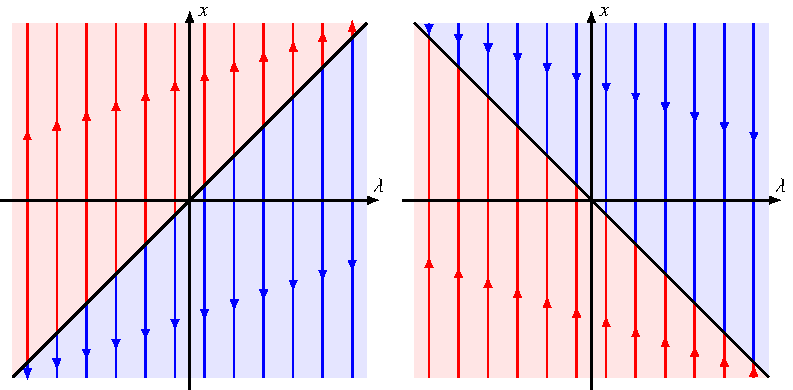
\includegraphics{chapters/3/lin1.pdf}
\caption{
Phasendiagramm der Differentialgleichung $\dot x = x-\lambda$ links und
$\dot x = -x-\lambda$ rechts.
Die Gleichgewichtslösung $x=\lambda$ ist im linken Fall instabil,
während $x=-\lambda$ im rechten Fall eine stabile Gleichgewichtslösung ist.
\label{skript:dgl:phasen1}
}
\end{figure}%
Der einfachste Fall ist bis auf eine Skalierung
\begin{equation}
f(x,\lambda)=x-\lambda.
\label{skript:dgl:linear1}
\end{equation}
$f$ hat nur einen einzigen kritischen Punkt, nämlich $x_0=-\lambda$.
Das Phasendiagramm dafür ist in Abbildung~\ref{skript:dgl:phasen1}
Man erkennt, dass Läsungen, die bei $x$-Werten $x>\lambda$ beginnen,
anwachsen und sich von der Gleichgewichtslösung entfernen.
Umgekehrt nehmen Lösungen ab, die bei $x$-Werten $x<\lambda$ beginnen,
und entfernen sich damit ebenfalls von der Gleichgewichtslösung.
Die Differentialgleichung mit rechter Seite~\ref{skript:dgl:linear1}
hat kein stabile Lösungen.

Die analoge Analyse für die Differentialgleichung
\[
\frac{dx}{dt} = -x-\lambda
\]
ist in Abbildung~\ref{skript:dgl:linear1} dargestellt.
Die Gleichgewichtslösung $x_0=-\lambda$ ist stabil.
\end{beispiel}

Dieses Beispiel zeigt, dass interessante Bifurkationsereignisse
erst dann auftreten, wenn der führende Term in $x$ der Taylor-Entwicklung
von $f$ von höherer als linearer Ordnung ist.


\subsection{Sattel-Knoten-Bifurkation}
\index{Sattel-Knoten-Bifurkation}%
\begin{figure}
\centering
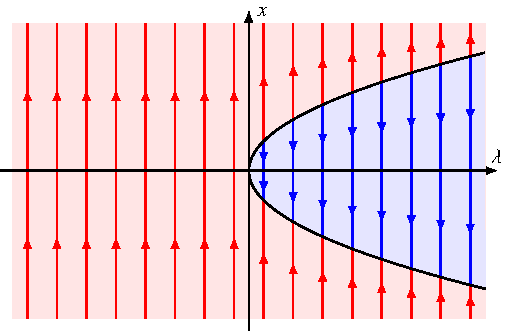
\includegraphics{chapters/3/saddle-node.pdf}
\caption{Phasendiagramm der Sattel-Knoten-Bifurkation zur
Differentialgleichung~\ref{skript:dgl:sattel-knoten-dgl}.
Für $\lambda>0$ gibt es zwei Gleichgewichtslösungen $\pm\sqrt{\lambda}$,
eine ist stabil, die andere instabil.
\label{skript:dgl:saddle-node}}
\end{figure}%
Die {\em Sattel-Knoten-Bifurkation}
\index{Sattel-Knoten-Bifurkation}%
tritt auf in der Differentialgleichung
\begin{equation}
\frac{dx}{dt}=x^2 - \lambda.
\label{skript:dgl:sattel-knoten-dgl}
\end{equation}
Für $\lambda >0$ hat die Gleichung~\ref{skript:dgl:sattel-knoten-dgl}
zwei Gleichgewichtslösungen $\pm\sqrt{\lambda}$.
In Abbildung~\ref{skript:dgl:saddle-node} ist das Phasendiagramm
dargestellt.
Daraus geht hervor, dass die Gleichgewichtslösung $q\sqrt{\lambda}$
instabil ist, während $-\sqrt{\lambda}$ stabil ist.

\subsection{Heugabel-Bifurkation}
\index{Heugabel-Bifurkation}%
\begin{figure}
\centering
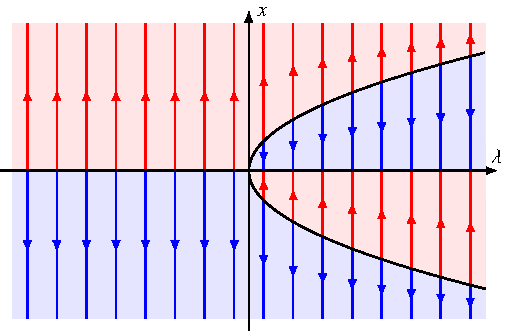
\includegraphics{chapters/3/pitchfork.pdf}
\caption{Phasendiagramm der Heugabel-Bifurkation.
\label{skript:dgl:pitchfork}}
\end{figure}
Die {\em Heugabel-Bifurkation} tritt bei der Differentialgleichung
\begin{equation}
\frac{dx}{dt} = x^3 - \lambda x
\label{skript:dgl:heugabel-dgl}
\end{equation}
auf, bei der der führende Term
dritter Ordnung in $x$ ist.
Die Differentialgleichung
kann auch in der Form
\[
\frac{dx}{dt}
=
x(x^2-\lambda)
\]
geschrieben werden.
Sie hat $0$ als Gleichgewichtslösung für alle $\lambda$.
Für $\lambda>0$ hat sie zusätzlich die Gleichgewichtslösungen
$\pm\sqrt{\lambda}$.

Das Phasendiagramm~\ref{skript:dgl:pitchfork} zeigt, dass
die einzige Gleichgewichtslösung bei $x_0=0$ instabil ist.
Beim Übergang zu $\lambda>0$ wird die Gleichgewichtslösung $x_0=0$
stabil.
Die beiden neuen Gleichgewichtslösungen $\pm\sqrt{\lambda}$ sind
beide instalbil.

Die Differentialgleichung
\[
\frac{dx}{dt} = -x^3+\lambda x
\]
hat die gleichen Gleichgewichtslösungen, jedoch ist $0$ für
$\lambda<0$ eine stabile Lösung, die beim Übergang zu $\lambda>0$
instabil wird.
Die Gleichgewichtslösungen $\pm\sqrt{\lambda}$ für $\lambda >0$
sind stabil.

\subsection{Transkritische Bifurkation}
\index{transkritische Bifurkation}%
\begin{figure}
\centering
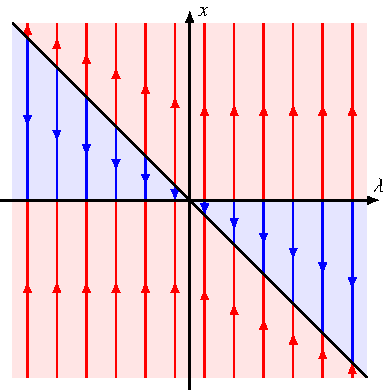
\includegraphics{chapters/3/trans.pdf}
\caption{Phasendiagramm der transkritischen Bifurkation in der
Differentialgleichung~\eqref{skript:dgl:transkritisch-dgl}.
\label{skript:dgl:transfig}}
\end{figure}
Die Differentialgleichung
\begin{equation}
\frac{dx}{dt}
=
x^2 + \lambda x
=
x(x+\lambda)
\label{skript:dgl:transkritisch-dgl}
\end{equation}
hat Gleichgewichtslösung $0$ und $-\lambda$.
Das Phasendiagramm in Abbildung~\ref{skript:dgl:transfig} zeigt, dass 
für $\lambda<0$ die Gleichgewichtslösung $0$ stabil ist, die
Gleichgewichtslösung $-\lambda$ hingegen instabil.
Beim Übergang zu $\lambda>0$ wird die Gleichgewichtslösung $0$ instabil
und die Gleichgewichtslösung $-\lambda$ wird instabil.

\subsection{Ein Beispiel zur globalen Mitteltemperatur\label{subsection:budyko}}
\index{globale Mitteltemperatur}%
\begin{figure}
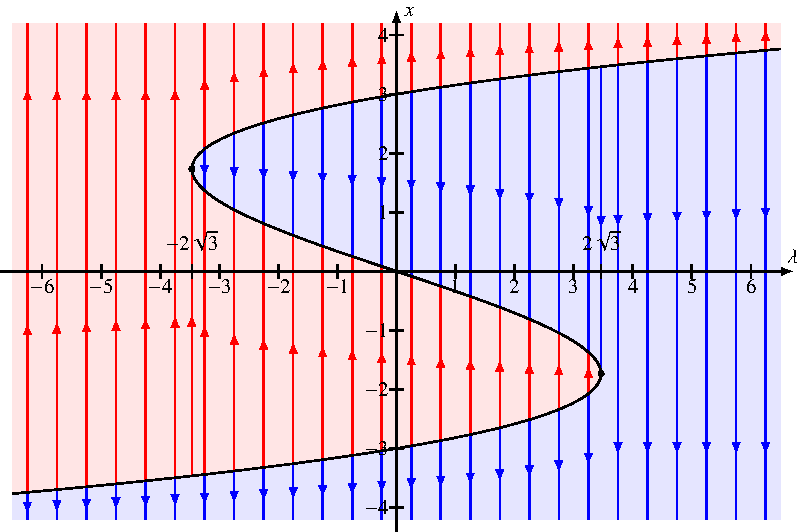
\includegraphics{chapters/3/kubisch.pdf}
\caption{Phasendiagramm der Differentialgleichung~\eqref{skript:dgl:kubisch}.
\label{skript:dgl:kubischfig}}
\end{figure}
Das in Abschnitt~\ref{subsection:modell von budyko} beschriebene
Budyko-Modell versucht, die globale Mittelemperatur in Abhängigkeit
von der Einstrahlung und der Albedo zu modellieren.
Mehr zu diesen Ansätzen wird in Kapitel~5 dargestellt.
\index{Budyko-Modell}

Als Beispiel für die Diskussion eines solchen Modells betrachten wir
die Differentialgleichung
\begin{equation}
\frac{dx}{dt}
=
\frac13(x^3 - 9x) - \lambda.
\label{skript:dgl:kubisch}
\end{equation}
Die Gleichgewichtslösungen sind die Nullstellen der kubischen Gleichung
\[
f(x,\lambda)
=
x^3-9x-3\lambda=0.
\]
Diese sind für beliebiges $\lambda$ nicht so leicht zu finden.
Für $\lambda=0$ sind die kritischen Punkte $0$ und $\pm 3$.
DIe Funktion $f(x)$ hat lokale Minima bei den $\pm\sqrt{3}$ mit
Funktionswerten $\pm2\sqrt{3}$.
Daher gibt es im Interval $(-2\sqrt{3},2\sqrt{3})$ drei 
Gleichgewichtslösungen, ausserhalb jedoch jeweils nur eine.

Das zugehörige Phasendiagramm ist in Abbildung~\ref{skript:dgl:kubischfig}
dargestellt.
Die Gleichgewichtslösungen oben und unten auf der S-Kurve sind instabil,
nur der Ast zwischen den beiden lokalen Extrema von $f(x)$ besteht
aus stabilen Gleichgewichtslösungen.

Wächst der Parameter $\lambda$ über den kritischen Wert $2\sqrt{3}$
hinaus, gibt es keinen stabilen Gleichgewichtszustand mehr, das System
divergiert nach $-\infty$. 
Analog strebt das System gegen $+\infty$ wenn der Parameter den Wert
$-2\sqrt{3}$ unterschreitet.

Die Differentialgleichung 
\begin{equation}
\frac{dx}{dt}
=
-f(x,\lambda)
\label{skript:dgl:kubisch2}
\end{equation}
hat die gleichen Gleichgewichtslösungen wie \eqref{skript:dgl:kubisch},
jedoch sind die stabilen Gleichgewichtslösungen von \eqref{skript:dgl:kubisch}
instabile Gleichgewichtslösungen von \eqref{skript:dgl:kubisch2}
und umgekehrt.
Beim Anstieg des Parameters $\lambda$ über den Wert $2\sqrt{3}$
springt das System, falls es sich im unteren Gleichtszustand befand,
in den oberen.
Sinkt der Wert von $\lambda$ wieder unter $2\sqrt{3}$ wird, bleibt
es jedoch auf dem oberen Gleichgewichtspunkt.



%
% lin.tex
%
% (c) 2018 Prof Dr Andreas Müller, Hochschule Rappreswil
%
\section{Linearisierung und Stabilität\label{section:linearisierung}}
\rhead{Linearisierung und Stabilität}
Die Technik der Phasendiagramme hat es sehr einfach gemacht, auf graphische
Art zwischen stabilen und instabilen Gleichgewichten zu unterscheiden.
Tatsächlich kann sie weiterentwickelt werden, in \cite{skript:mathsem-dgl}
wird gezeigt, wie man Gleichgewichtslösungen auch zweidimensionaler
Systeme ganz ähnlich graphisch analysieren kann.
In diesem Abschnitt soll aber nur gezeigt werden, wie auch mit relativ
bescheidenem Aufwand auch auf algebraischem oder analytischem Weg
Aussagen über die Stabilität von Gleichgewichtslösungen gefunden werden
können.

\subsection{Lineare Differentialgleichungen}
Eine lineare Differentialgleichung
\index{lineare Differentialgleichung}%
\begin{equation}
\frac{dx}{dt}
=
Ax
\label{skript:lin:dgl}
\end{equation}
kann mit der Matrix-Exponentialfunktion
\begin{equation}
x(t) = e^{At} x(0)
=
\biggl(
\sum_{k=0}^\infty \frac{t^k}{k!}A^k
\biggr)\, x(0)
=
\biggl(
1+ At + \frac{A^2t^2}{2!} +\frac{A^3t^3}{3!}+\dots
\biggl)\mathstrut\cdot x(0)
\label{skript:lin:potenzreihe}
\end{equation}
gelöst werden.

Für eine diagonalisierbare Matrix $A$ ist die Berechnung der
Potenzreihe~\eqref{skript:lin:potenzreihe} sehr viel einfacher, da
gilt
\begin{equation}
A^k
=
\begin{pmatrix}
\lambda_1&\dots &0        \\
\vdots   &\ddots&\vdots   \\
0        &\dots &\lambda_n
\end{pmatrix}^k
=
\begin{pmatrix}
\lambda_1^k&\dots &0        \\
\vdots     &\ddots&\vdots   \\
0          &\dots &\lambda_n^k
\end{pmatrix}
\qquad\Rightarrow\qquad
e^{tA}
=
\begin{pmatrix}
e^{\lambda_1 t} & \dots  & 0             \\
\vdots          & \ddots &\vdots         \\
0               & \dots  &e^{\lambda_n t}
\end{pmatrix}.
\label{skript:lin:expreihe}
\end{equation}
Insbesondere lässt sich damit sehr einfach entscheiden, ob wie Lösungen
für zunehmendes $t$ anwachsen oder gegen $0$ konvergieren.
Ist $\lambda_j = a_j + ib_j$ die Aufteilung in Real- und Imaginärteil,
dann ist
\[
e^{\lambda_jt} = e^{a_jt}(\cos b_jt +i\sin b_jt)
\qquad\Rightarrow\qquad
|e^{\lambda_j t}| = e^{a_jt}.
\]
Ist $a_j < 0$, dann konvergiert $e^{\lambda_jt}$ gegen $0$.
Da die $0$-Lösung eine Gleichgewichtslösung von~\eqref{skript:lin:dgl}
ist, kann gefolgert werden, dass diese Lösung genau dann stabil ist, 
wenn alle Eigenwerte von $A$ negativen Realteil haben.

Natürlich lässt sich nicht jede Matrix diagonalisieren, aber man kann
mindestens eine Basis finden, in der $A$ Jordan-Normalform hat, also aus
\index{Jordan-Normalform}%
Blöcken der Form
\[
A_{\lambda}
=
\begin{pmatrix}
\lambda&   1   &       &       &       \\
       &\lambda&   1   &       &       \\
       &       &\lambda&\ddots &       \\
       &       &       &\ddots &    1  \\
       &       &       &       &\lambda
\end{pmatrix}
=
\begin{pmatrix}
\lambda&       &       &       \\
       &\lambda&       &       \\
       &       &\ddots &       \\
       &       &       &\lambda
\end{pmatrix}
+
\begin{pmatrix}
   0   &   1   &       &       \\
       &   0   &\ddots &       \\
       &       &\ddots &   1   \\
       &       &       &   0
\end{pmatrix}
=
\lambda E + N.
\]
Die Matrizen $\lambda E$ und $N$ vertauschen, so dass die
Produkteigenschaft der Exponentialfunktion verwendet werden kann,
es gilt
\begin{equation}
e^{A_\lambda t}
=
e^{\lambda tE}\cdot e^{Nt}
=
e^{\lambda t} e^{Nt}.
\label{skript:lin:faktorisierung}
\end{equation}
Bezeichnet man mit $N_i$ die Matrix, die in der $i$-ten Nebendiagonale
Einsen enthält und sonst nur Nullen, dann ist $N=N_1$.
Die Potenzen von $N$ können dann sofort in der Form $N^k=N_k$ ausgedrückt
werden, und damit kann man auch
\begin{equation}
e^{Nt}
=
\begin{pmatrix}
1&t&\frac{t^2}{2!}&\frac{t^3}{3!}& \dots & \frac{t^{n-1}}{(n-1)!}\\
0&1&       t      &\frac{t^2}{2!}& \dots & \frac{t^{n-2}}{(n-2)!}\\
      &\ddots&\ddots& \ddots     &       & \vdots                \\
      &      &\ddots& \ddots     &\ddots & \vdots                \\
      &      &      &         0  &    1  & t \\
      &      &      &            &    0  & 1
\end{pmatrix}
=
\sum_{k=0}^{n-1} \frac{t^k}{k!}N_k
\end{equation}
sofort berechnen.
Der Faktor $e^{Nt}$ von \eqref{skript:lin:faktorisierung}
hängt nicht von $\lambda$ ab und wächst höchstens mit $t^{n-1}$ an.
Dies bedeutet, dass das Stabilitätskriterium an die Eigenwerte von $A$
weiterhin zutrifft: Die Gleichgewichtslösung $x=0$ ist genau dann stabil,
wenn alle Eigenwerte von $A$ negativen Realteil haben.

\subsection{Linearisierung\label{subsection:linearisierung}}
Ist $x_0$ ein kritischer der Punkt der autonomen Differentialgleichung
\[
\frac{dx}{dt} = f(x),
\]
dann können wir mit Hilfe einer Koordinatentransformation
\[
x = x_0 + \tilde x
\qquad
\text{und}
\qquad
\tilde f(\tilde x) = f(x_0 + \tilde x)
\]
die Differentialgleichung in die Form
\[
\frac{d\tilde x}{dt}
=
\tilde f(\tilde x)
\]
bringen, welche $0$ als Gleichgewichtslösung hat.
Im Folgenden schreiben wir wieder $f$ und $x$ für $\tilde f$ und $\tilde x$.

Da $f(0)=0$ gilt, kann $f(x)$ in eine Potenzreihe der Form
\[
f(x) = Ax + O(|x|^2)
\]
entwickelt werden.
Darin ist $A$ die Ableitungsmatrix
\[
A=(a_{ij})=Df
\qquad\text{mit}\qquad
(Df)_{ij}
=
\frac{\partial f_i(x)}{\partial x_j} = a_{ij}
\]
der Funktion $f$.
Dies ist die {\em linearisierte} Version der
\index{linearisierte Differentialgleichung}%
Differentialgleichung~\eqref{skript:lin:dgl}.

In unmittelbarer Nähe des Gleichgewichtspunktes $0$ sind analog wie
bei der linearen Differentialgleichung~\eqref{skript:lin:dgl}
wieder die Eigenwerte der Matrix $A=Df$ darüber entscheidend, ob der
Gleichgewichtspunkt stabil ist.
$x_0$ ist genau dann ein stabiler Gleichgewichtspunkt, wenn alle
Eigenwerte der Ableitungsmatrix $Df$ negativ sind.










\section*{Übungen}
\begin{uebungsaufgaben}
\item
Betrachten Sie die Differentialgleichung
\begin{equation}
\frac{dx}{dt}
=
x^4-4x^2-\lambda
\label{aufgabe301:gl}
\end{equation}
\begin{teilaufgaben}
\item
Finden Sie die Gleichgewichtslösungen und untersuchen Sie die 
Bifurkationen, die bei Veränderungen des Parameters $\lambda$
auftreten können.
\item
Welche Gleichgewichtslösung wird das System einnehmen, wenn der
Parameter $\lambda$ erst von $-1$ auf $1$ anwächst
und dann wieder auf $-1$ absinkt.
\end{teilaufgaben}

\begin{loesung}
\begin{figure}
\centering
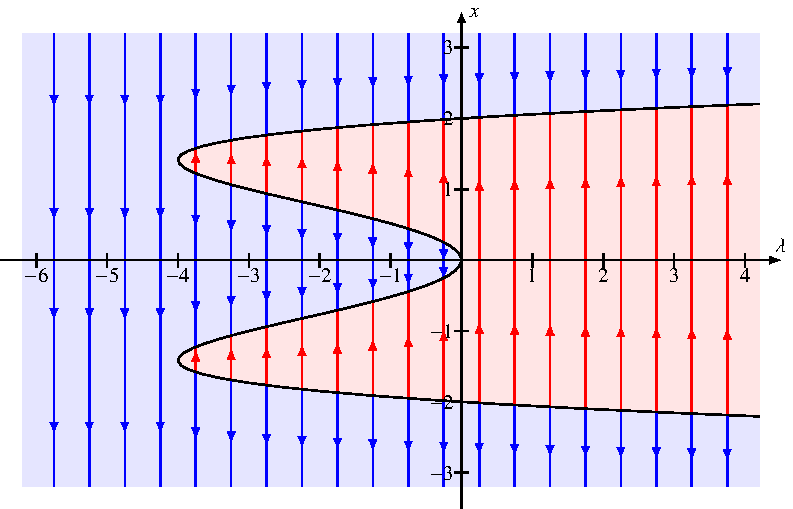
\includegraphics{chapters/3/grad4.pdf}
\caption{Phasendiagramm der Differentialgleichung~\eqref{aufgabe301:gl}.
\label{aufgabe301:fig}}
\end{figure}
\begin{teilaufgaben}
\item
Die kritischen Punkte der Differentialgleichung~\eqref{aufgabe301:gl}
sind Nullstellen der Gleichung
\begin{equation}
x^4-4x^2-\lambda=0
\label{aufgabe301:nullstellen}
\end{equation}
Dies ist eine quadratische Gleichung in $x^2$, die mit der Lösungsformel
für die quadratische Gleichung gelöst werden kann:
\[
x^2 = 2 \pm \sqrt{4+\lambda}.
\]
Diese Gleichung hat reelle Lösungen für $\lambda \ge -4$.
Für $\lambda \le 0$ ist die Quadratwurzel nicht grösser als $2$,
so dass die beiden Nullstellen positiv sind, es also vier verschiedene
Lösungen
\begin{equation}
x_{1,2,3,4} = \pm\sqrt{2\pm\sqrt{4+\lambda}}
\end{equation}
hat.
Für $\lambda >0$ hat die quadratische Gleichung eine negative Lösung
für $x^2$, die also nicht zu einer reellen Lösung der
Gleichung~\eqref{aufgabe301:nullstellen} führen kann.
Nur aus der positive Lösung $2+\sqrt{4+\lambda}$ kann man eine
Gleichgweichslösung, nämlich
\[
x=\pm\sqrt{2+\sqrt{4+\lambda}}
\]
ableiten.
Für $\lambda < -4$ gibt es gar keine Gleichgewichtslösung.

Das Phasendiagramm in Abbildung~\ref{aufgabe301:fig} zeigt,
dass für $\lambda >0$ die obere Gleichgewichtslösung stabil ist,
untere dagegen instabil.
Für $-4\le\lambda\le 0$ sind die Gleichgewichtslösungen
\begin{align*}
&\sqrt{2+\sqrt{4+\lambda}}
&&\text{und}&
&-\sqrt{2-\sqrt{4+\lambda}}
\\
\intertext{stabil und die Gleichgewichtslösungen}
&-\sqrt{2+\sqrt{4+\lambda}}
&&\text{und}&
&\sqrt{2-\sqrt{4+\lambda}}
\end{align*}
instabil.

Bei $\lambda=-4$ finden gleichzeitig zwei Sattel-Knoten-Bifurkationen 
statt, bei $\lambda=0$ findet ein einfache Sattel-Knoten-Bifurkation
statt, jedoch in umgekehrter Richtung wie im Beispiel im Text.
\item
Beim Anwachsen des Parameters über den Punkt $\lambda=0$ springt die
Gleichgewichtslösung auf die stabile Lösung
\[
x(\lambda)=\sqrt{2+\sqrt{4+\lambda}}.
\]
Bei der anschliessenden Verringerung von $\lambda$ bleibt die 
Gleichgewichtslösung auf dem Ast $x(\lambda)$ der Kurve, da diese
alle stabil sind.
Unabhängig vom Ausgangszustand befindet sich das System am Ende des
beschriebenen Szenarios also immer in der Nähe der Gleichgewichtslösung
\[
x(-1)=\sqrt{2+\sqrt{3}}.
\qedhere
\]
\end{teilaufgaben}
\end{loesung}


\end{uebungsaufgaben}

